% ==========================================================================
% Figure blocks for
%   Biological Catalysis Mechanisms
%
% Each block below is self-contained. Paste one straight into
% the manuscript at the point its panel belongs; no \input and
% no \captionPanel* macro is required.
%
% Preamble requirements:
%   \usepackage{graphicx}
%   \usepackage{amsmath,amssymb}
%   \graphicspath{{figures/}}      % if the paths below are bare
%
% These captions contain no cross-references, so the blocks
% compile in any document that can show a figure.
% ==========================================================================


% --------------------------------------------------------------------------
\begin{figure*}[!htbp]
    \centering
    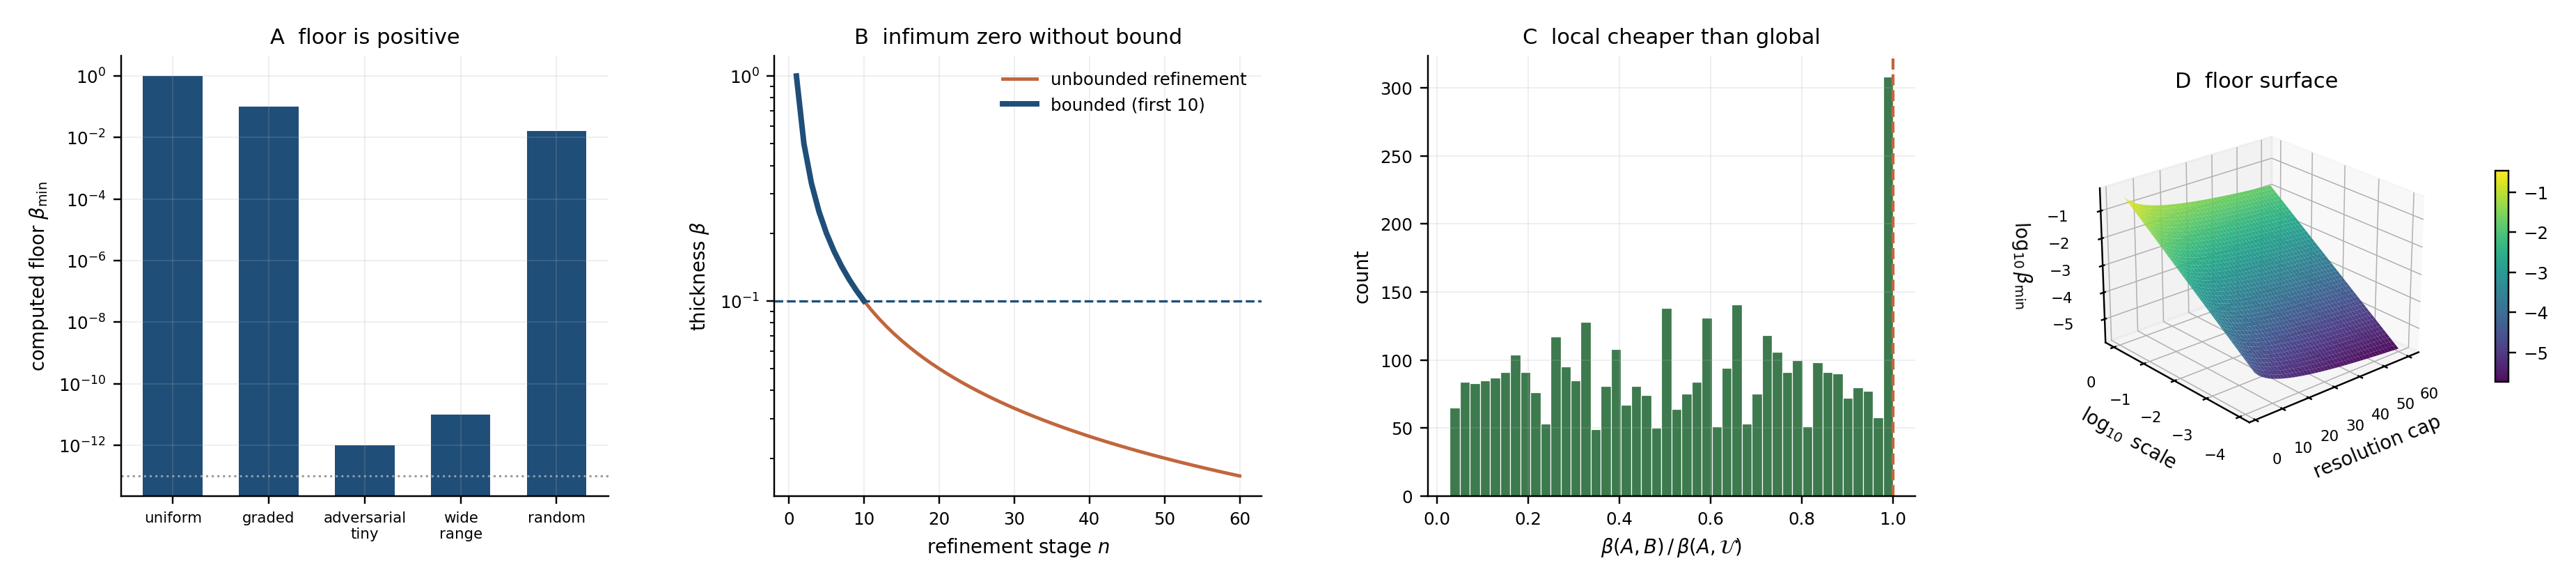
\includegraphics[width=\textwidth]{figures/panel_01.png}
    \caption{\textbf{Individuation is not free: positivity of the boundary
    thickness and the hypothesis its uniformity requires.}
    \textbf{(A)}~Contact floor $\beta_{\min}$ computed---not assumed---as the
    minimum edge weight over five resolution-bounded structures spanning twelve
    orders of magnitude, including an adversarial instance whose smallest weight is
    $10^{-12}$. Every instance returns a strictly positive floor; the dotted
    reference marks $10^{-13}$. Positivity does not depend on the scale of the
    weights.
    \textbf{(B)}~Thickness against refinement stage for a system permitted to refine
    without limit (orange), generating the sequence $1/n$. Each term is strictly
    positive and the sequence has infimum zero: every $\varepsilon$ in a ladder down
    to $10^{-9}$ is eventually cleared. Truncating the same sequence to a
    resolution-bounded system (blue, first ten stages) restores a positive floor at
    $0.1$ (dashed). Uniformity of the floor therefore requires the
    resolution-boundedness hypothesis and is not unconditional.
    \textbf{(C)}~Distribution of the ratio $\beta(A,B)/\beta(A,\mathcal{U})$ over
    $4000$ randomly generated nested structures. The ratio never exceeds unity
    (dashed), confirming that distinguishing an item from a specific finite partner
    costs no more than distinguishing it from the totality. Contact is the
    cheaper way to be distinct.
    \textbf{(D)}~Floor surface $\log_{10}\beta_{\min}$ over the resolution cap and
    the weight scale. The surface is strictly negative-valued but nowhere reaches
    $-\infty$: for any finite cap the floor is bounded away from zero, and it
    descends toward zero only as the cap is removed. The two controlling variables
    act independently, the cap setting how finely the system may divide and the
    scale setting the size of the smallest available distinction.}
    \label{fig:panel1}
\end{figure*}


% --------------------------------------------------------------------------
\begin{figure*}[!htbp]
    \centering
    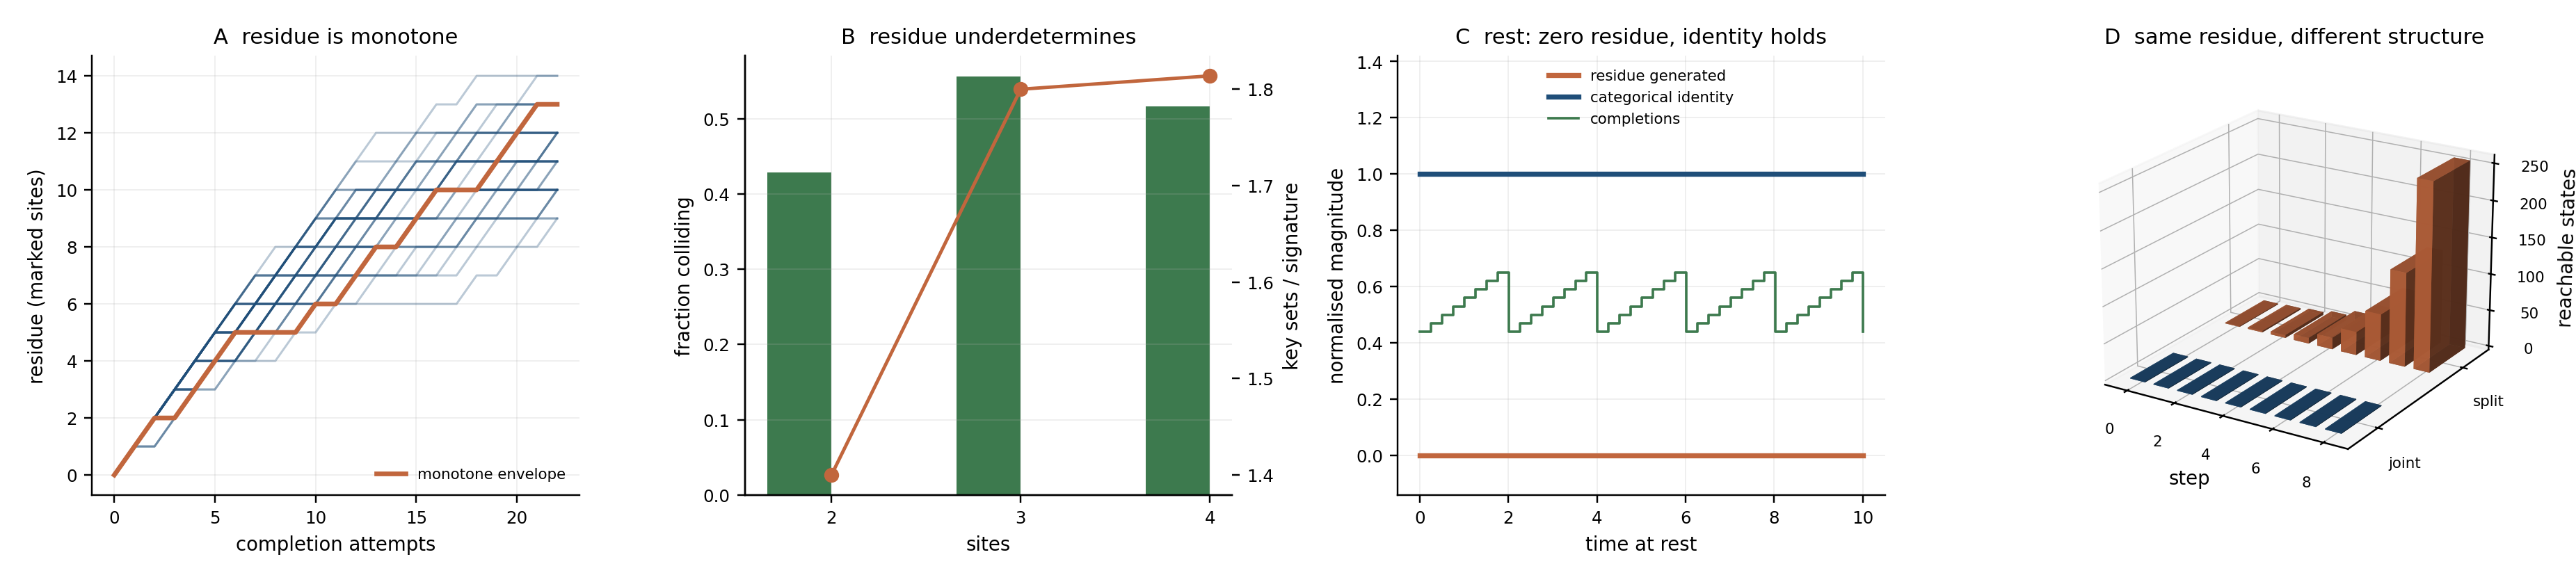
\includegraphics[width=\textwidth]{figures/panel_02.png}
    \caption{\textbf{Category and residue are independent primitives, and the
    independence is exhibited at zero residue.}
    \textbf{(A)}~Forty independent trajectories of the abstract system, each
    attempting completions at randomly chosen sites over fourteen sites. Residue,
    measured as the number of marked sites, is non-decreasing along every
    trajectory: attempts on already-marked sites are no-ops and no operation
    unmarks. The monotone envelope is shown in orange. Irreversibility is a
    property of the accumulation, not of any individual step.
    \textbf{(B)}~Exhaustive enumeration over all key sets of size at most three on
    two to four sites. Green bars give the fraction of key sets that share a
    terminal residue signature with at least one other key set; the orange curve
    gives the mean number of distinct key sets per signature. Distinct categorical
    structures routinely leave identical residue, so a record of what was resolved
    does not determine the capacities that did the resolving.
    \textbf{(C)}~The limiting case. For a configuration admitting no applicable key,
    residue generated is identically zero (orange) for all time, while the
    categorical identity is invariant and fully determined (blue) and completions
    continue (green). A quantity that vanishes where another is fully engaged
    cannot be that other quantity. This is the separation of the two primitives at
    zero residue, and it requires no process to occur.
    \textbf{(D)}~Reachable-state growth for two systems with identical terminal
    residue but different categorical structure: a single joint key that marks two
    sites at once, and two split keys that mark one site each. The split structure
    reaches exponentially more intermediate states. Terminal residue is blind to
    this difference; the reachable set is not.}
    \label{fig:panel2}
\end{figure*}


% --------------------------------------------------------------------------
\begin{figure*}[!htbp]
    \centering
    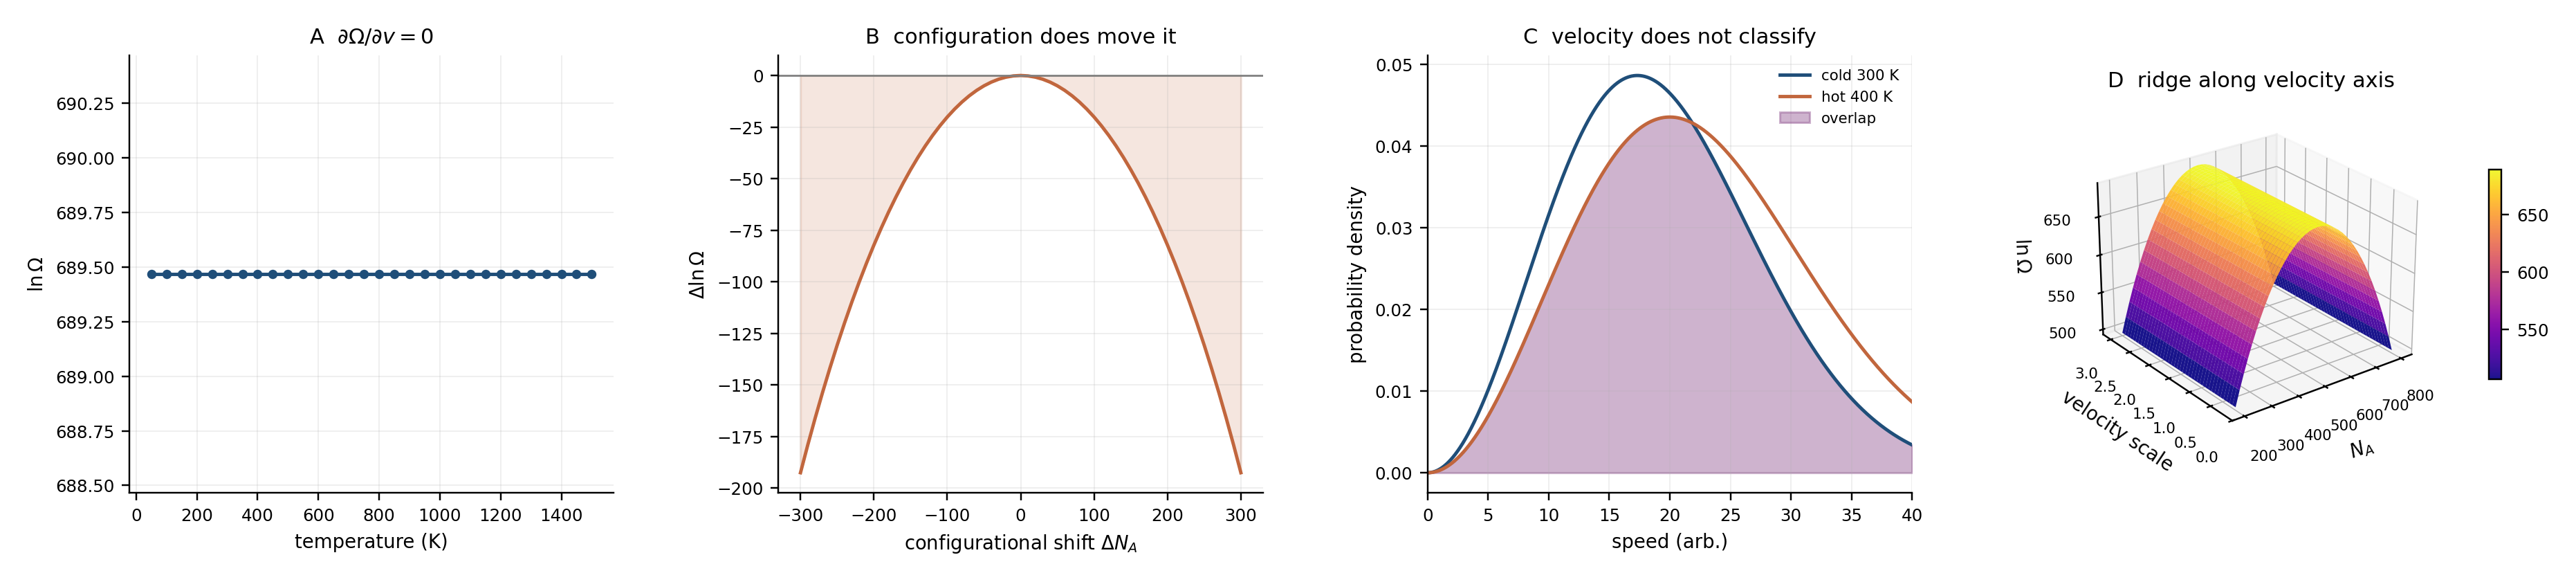
\includegraphics[width=\textwidth]{figures/panel_03.png}
    \caption{\textbf{Configurational and kinetic quantities depend on disjoint
    variables, and the statistic that shows it is not blind.}
    \textbf{(A)}~$\ln\Omega$ computed from occupation numbers while velocities are
    resampled from Maxwell--Boltzmann distributions at thirty temperatures from
    $50$ to $1500$\,K, at fixed configuration. The value does not move: the spread
    is identically zero to machine precision, giving $\partial S/\partial v = 0$
    numerically. The vertical axis is expanded by two units about the value to make
    the absence of variation visible.
    \textbf{(B)}~The discriminating control. The same statistic under
    \emph{configurational} perturbation, shifting $\Delta N_A$ from $-300$ to
    $+300$ at fixed total. $\ln\Omega$ moves by nearly two hundred units. Without
    this panel (A) would be consistent with a constant statistic and would carry no
    information; with it, (A) is a statement about velocity specifically.
    \textbf{(C)}~Maxwell--Boltzmann speed distributions at $300$\,K and $400$\,K
    with the overlap region shaded. The distributions overlap over most of their
    support, so a single speed does not identify which ensemble a molecule came
    from. Threshold sorting on velocity performs only marginally above chance.
    \textbf{(D)}~$\ln\Omega$ over the configurational coordinate $N_A$ and a
    velocity scale. The surface is a ridge: strongly curved along the
    configurational axis and exactly flat along the kinetic one. A device that
    manipulates the flat coordinate cannot move the height, which is the geometric
    content of the orthogonality result.}
    \label{fig:panel3}
\end{figure*}


% --------------------------------------------------------------------------
\begin{figure*}[!htbp]
    \centering
    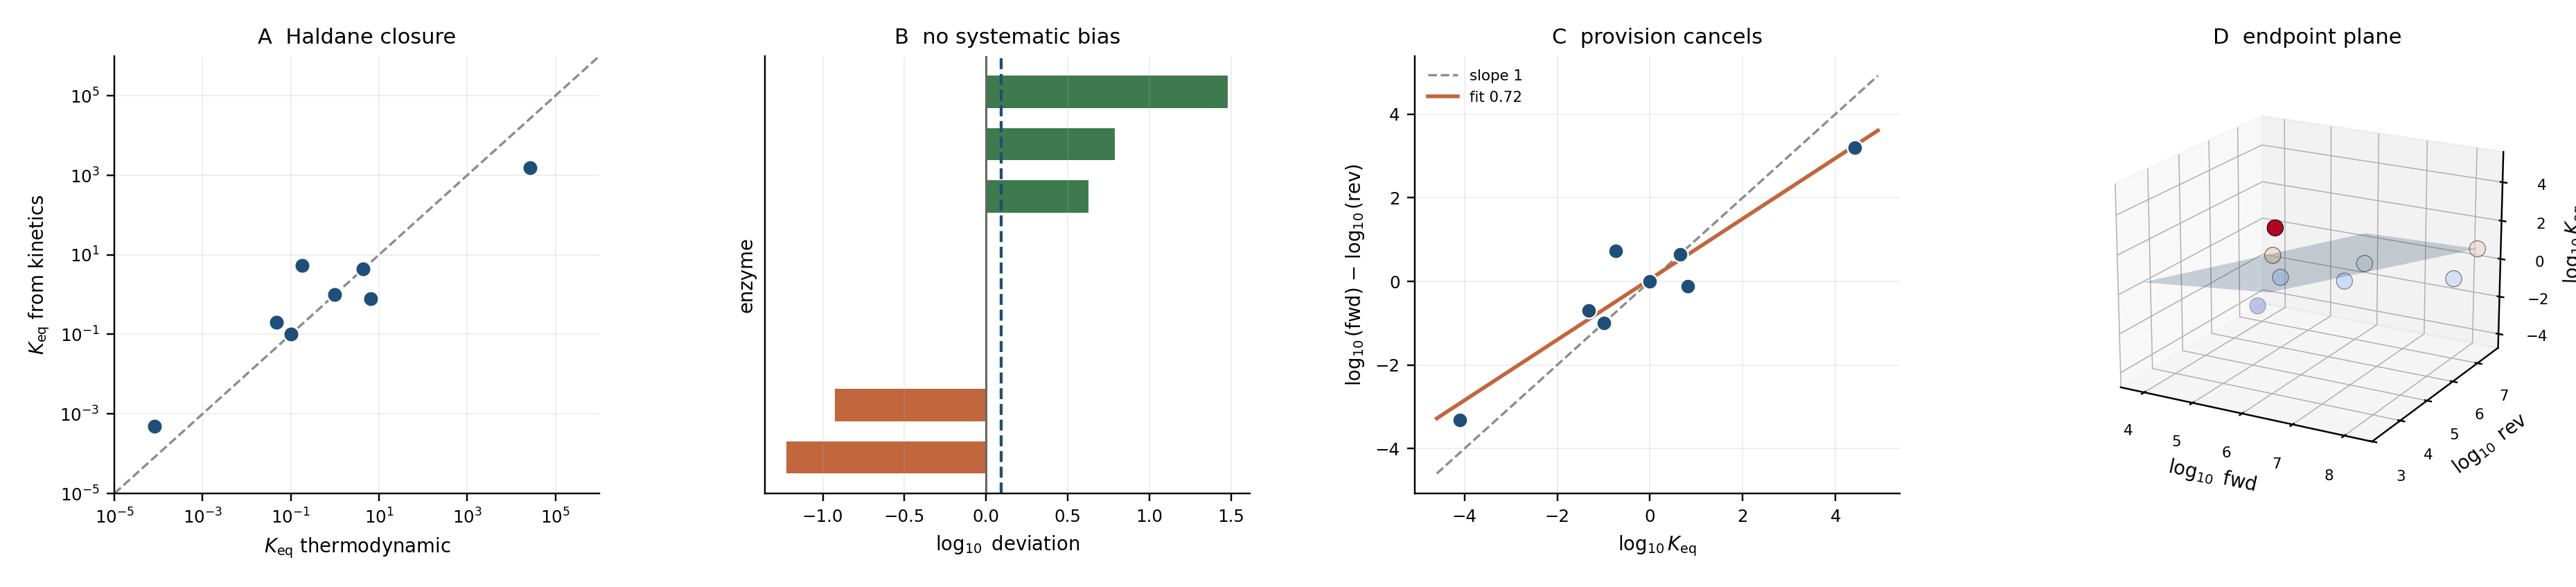
\includegraphics[width=\textwidth]{figures/panel_04.png}
    \caption{\textbf{The catalyst supplies categories to the transition and not to
    the endpoints: equilibrium invariance and the Haldane relation.}
    \textbf{(A)}~Equilibrium constant reconstructed from forward and reverse
    kinetic parameters against the independently measured thermodynamic value, for
    eight reversible enzymes, over eleven orders of magnitude. Points scatter about
    the identity line (dashed) without systematic displacement.
    \textbf{(B)}~Per-enzyme $\log_{10}$ deviation of the kinetic from the
    thermodynamic constant, sorted. Deviations fall on both sides of zero; the mean
    (dashed blue) is $0.094$ decades, giving $t = 0.30$ against zero bias. The
    theorem forbids a systematic catalyst-dependent shift, not scatter, and it is
    the mean rather than the spread that is diagnostic---the spread reflects the
    heterogeneity of literature conditions.
    \textbf{(C)}~The sharper form of the test. The difference of forward and reverse
    log-efficiencies against $\log_{10}K_{\mathrm{eq}}$, with the unit-slope
    reference (dashed) and the fitted line (orange, slope $0.72$), $r = 0.948$. If
    provision is a property of the transition it is common to both directions and
    cancels in the ratio, leaving only the endpoint term. A permutation control over
    $20{,}000$ shuffles gives $p = 2.5\times10^{-4}$.
    \textbf{(D)}~Forward efficiency, reverse efficiency and equilibrium constant for
    the same eight enzymes, with the plane $z = x - y$ overlaid. The points lie on
    the plane, which is the geometric statement of the Haldane relation: the
    equilibrium constant is the difference of the two efficiencies and carries no
    independent contribution from the catalyst.}
    \label{fig:panel4}
\end{figure*}


% --------------------------------------------------------------------------
\begin{figure*}[!htbp]
    \centering
    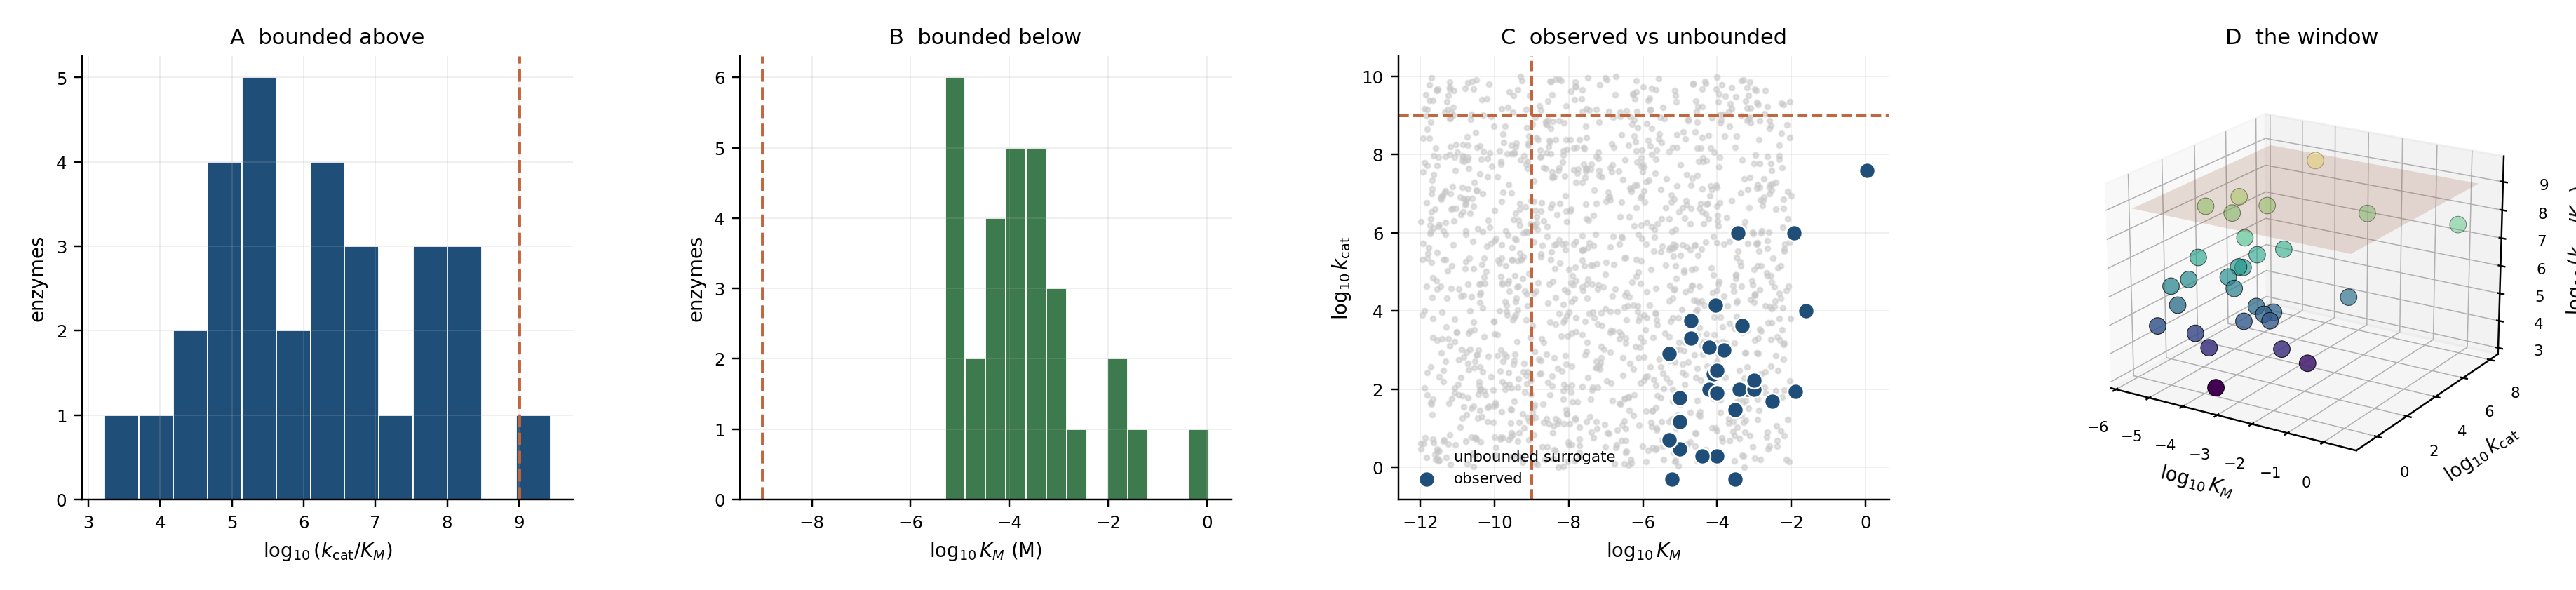
\includegraphics[width=\textwidth]{figures/panel_05.png}
    \caption{\textbf{Specificity is bounded on both sides: provision sets a floor,
    release sets a ceiling.}
    \textbf{(A)}~Distribution of catalytic efficiency over thirty characterised
    enzymes spanning six decades. No entry exceeds the diffusion limit (dashed),
    and the mass of the distribution sits well below it. Efficiency is bounded above
    by more than diffusion alone.
    \textbf{(B)}~Distribution of $K_M$ for the same enzymes. No catalytically
    competent entry has $K_M$ below $1$\,nM (dashed). Binding tight enough to
    compromise release does not occur among enzymes that turn over, which is the
    release bound of the specificity-window theorem.
    \textbf{(C)}~The window in the $K_M$--$k_{\mathrm{cat}}$ plane. Grey points are
    the surrogate distribution that would falsify the claim---efficiency uniform to
    the diffusion ceiling, affinity unbounded below---and blue points are the
    observed enzymes. The observed set occupies a bounded interior region while the
    surrogate fills the plane. Without the surrogate a bounded sample would be
    uninformative; with it, the bound is a finding.
    \textbf{(D)}~The same enzymes in three dimensions, with efficiency as the
    vertical coordinate and the diffusion ceiling drawn as a plane. The occupied
    volume is bounded on the affinity axis, on the turnover axis, and beneath the
    ceiling. The interior optimum is a consequence of two independent requirements
    acting in opposite directions, not of optimisation toward a target.}
    \label{fig:panel5}
\end{figure*}


% --------------------------------------------------------------------------
\begin{figure*}[!htbp]
    \centering
    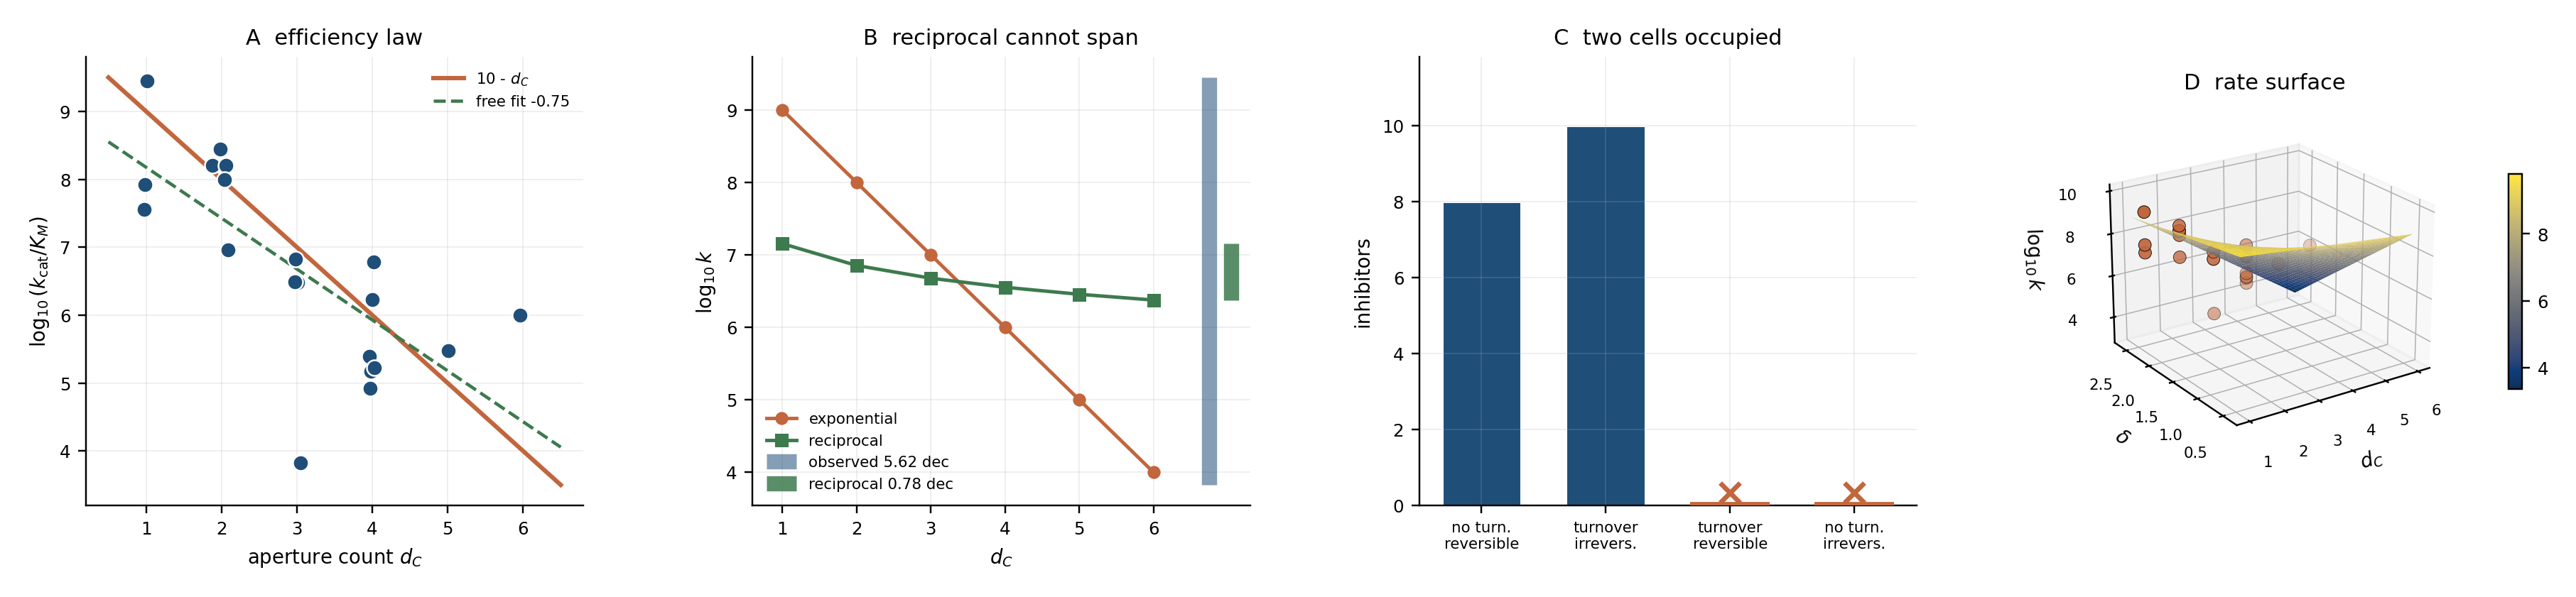
\includegraphics[width=\textwidth]{figures/panel_06.png}
    \caption{\textbf{Aperture counting predicts efficiency with one global
    constant; the reciprocal law is excluded on dynamic range; inhibition occupies
    exactly two of four cells.}
    \textbf{(A)}~Catalytic efficiency against aperture count $d_C$, assigned from
    documented mechanisms by the simultaneity rule without reference to measured
    rates. The parameter-free law $\log_{10}(k_{\mathrm{cat}}/K_M) = 10 - d_C$
    (orange) is drawn with no fitted quantity; the free two-parameter fit (green
    dashed) returns slope $-0.75$ and improves the mean absolute error by only
    $5.6\%$. Points are jittered horizontally for visibility. Permuting $d_C$ across
    enzymes gives $p = 4\times10^{-4}$.
    \textbf{(B)}~The exclusion of the reciprocal alternative. The exponential law
    (orange) and the reciprocal law $k \propto 1/(d_C\tau)$ (green) over the
    documented range $d_C = 1$--$6$, with the representable spans drawn as vertical
    bars at right. The observed efficiencies span $5.62$ decades; the reciprocal
    law can span at most $\log_{10}6 = 0.78$ decades whatever $\tau$ is chosen,
    since $\tau$ enters as a common factor and cancels. The exclusion is arithmetic
    and does not depend on fit quality.
    \textbf{(C)}~The inhibition dichotomy. Nineteen documented inhibitors
    classified on two independently determined experimental axes---whether
    inactivation requires catalytic turnover, and whether activity is recovered on
    dilution. Two cells are occupied ($8$ competitive, $10$ mechanism-based); the
    two cells the theorem forbids are empty, marked with crosses. Permuting the
    reversibility labels fills on average $3.999$ of the four cells,
    $p = 4\times10^{-5}$.
    \textbf{(D)}~Rate surface over aperture count and depth increment $\delta$, with
    the observed enzymes overlaid at $\delta = \ln 10$. The surface descends
    linearly in $d_C$ at fixed $\delta$; the observed points track that descent. The
    single global constant is the intercept, and no per-enzyme freedom is used.}
    \label{fig:panel6}
\end{figure*}

